%
%  愛知工業大学 情報科学部 情報科学科
%    要旨集用LaTeXテンプレート(2016.11.28)
%
%  original by Nobuhiro Ito
%  revised by Susumu Suzuki & Masashi Morimoto on 2016.11.28
%
\documentclass{jarticle}
\pagestyle{empty}

%% レイアウト
\setlength{\topmargin}{-10.4mm}
\setlength{\headheight}{0mm}
\setlength{\headsep}{0mm}
\setlength{\textheight}{262mm}
\setlength{\textwidth}{180mm}
%\setlength{\topskip}{7mm}
\setlength{\evensidemargin}{-10.4mm} 
\setlength{\oddsidemargin}{-10.4mm} 
\setlength{\columnsep}{8mm}

%% パッケージ環境
% graphicx: 画像読み込み
%  dvipdfmxをドライバ指定することでpdf/png/jpeg形式の図を利用可能
%  異なるドライバを利用する場合はそのドライバ指定に変更
% \usepackage{graphicx} % suzuki
\usepackage[dvipdfmx]{graphicx} % suzuki
% subcaption: subfigureを置き換えたパッケージ(複数の図用)
% \setlength{\footskip}{12mm}
% \usepackage{subfigure}	 % suzuki
\usepackage{subcaption} % suzuki
% color:文章に色をつけたいとき
%  利用例:\textcolor{red}{文章}
% \usepackage{color}
\usepackage{booktabs}
\usepackage{setspace}

% 行間調整
\setstretch{0.9}

%sectionのフォントサイズ修正
\makeatletter
\def\section{\@startsection {section}{1}{\z@}{2.5ex plus -1ex minus -.2ex}{1.3 ex plus .1ex}{\large\bf}}
\makeatother 

%subsectionのフォントサイズ修正
\makeatletter
\def\subsection{\@startsection {subsection}{1}{\z@}{1.5ex plus -1ex minus -.4ex}{0.3 ex plus .1ex}{\bf}}
\makeatother 

\begin{document}
\twocolumn[

  \begin{center}
    %タイトル
    {\LARGE \textbf{独立したコミュニティにおける滞在ウォッチの安定運用のためのシステム拡張に関する研究}}\\
    %サブタイトル
    %{\Large \textbf{必要に応じてサブタイトル}}
  \end{center}

  \begin{center}
    % 著者
    \begin{tabular}{cccc}
      % 1名の場合
      %\multicolumn{4}{c}{K11001 愛工総和}\\
      % 2名の場合
      %& K11002 愛工七音 & X11003 愛工頼音 &\\
      % 3名の場合
      %K11001 愛工総和 & K11002 愛工今鹿 & X11003 愛工姫星&\\
      % 4名の場合
      K19074 外山瑠起 & k190 \\
      % 指導教員
      \multicolumn{4}{c}{\textbf{指導教員} 梶克彦}
    \end{tabular}
    \hspace{2zw}
  \end{center}
]

%--------------------------------------------
\section{はじめに}
\label{sec:intro}
研究室やコワーキングスペースのような場所では部屋利用者の在室情報が分かると様々な応用ができる.部屋の利用者数や時間帯が把握できれば,環境整備や活用状況が少ない部屋の省エネ化の指標となる.また目的とする人の居場所を把握できれば,コミュニケーションの円滑化や共同作業を支援できる.

しかし研究室のような場所では必ずしも在室情報が記録されているとは限らない.またコアタイムが存在しないような研究室では常に活発なコミュニケーションがあるとは限らない
在室者を検出する方法としてスマートフォンやビーコンを用いた検出方法がある [1].スマートフォンとビーコンを利用し,在室者を検出する手法である.
しかし,部屋利用者が能動的に記録をしないといけないという問題点がある.また会社において気軽なコミュニケーション促進を目的とした研究がある [2].しかし,システムの導入が会社におけるものなので研究室での環境に適合しないと考える.

そこで我々の先行研究として BLE ビーコンを用いた在室管理プラットフォーム「滞在ウォッチ」が提案されている.滞在ウォッチでは利用者の負担軽減のために,在室者情報を BLEビーコンで受動的に記録する方法を採用されている.
在室管理プラットフォームの概要を図 1 に示す.ビーコンを持った利用者が部屋に訪れると受信機が検知し,サーバに在室者情報を送信しデータベースに記録する.
データベースに保存された情報は独自に作成したAPIによって外部からの利用が可能である.
過去の研究として滞在ウォッチAPIを用いた退勤管理システムや在室状況可視化システム,部屋利用者の来訪促進システム,コミュニケーション促進システムなど様々な応用システムの構築がされてきた.[4][5]

この滞在ウォッチの複数コミュニティ間での連携を考えている.ここでいう複数コミュニティ間とは物理的な距離が近く,同じようなことをやっているコミュニティ間と定義する.複数コミュニティ間で滞在ウォッチを連携したい理由としてこのようなコミュニティ間でコミュニケーション促進できれば知見の共有や新規性のある想像ができる可能性高いからである.

しかし滞在ウォッチは単一コミュニティでの運用を前提なため複数コミュニティ間で連携するには複数の問題点が存在する.各コミュニティで独立した運用ができていない,受信機のデータ精度が高くない,色んな属性の人が継続的に利用できない,継続的なメンテナンスが困難な点が上げられる.上記の問題を解決しなければ複数のコミュニティ間で連携することは難しい.これらの問題を解決した滞在ウォッチの運用を安定運用と定義する.
本研究では滞在ウォッチを複数コミュニティ間で連携するために独立したコミュニティにおける滞在ウォッチの安定運用のためのシステム拡張について提案する.


\begin{figure}[tbh]
  \centering
  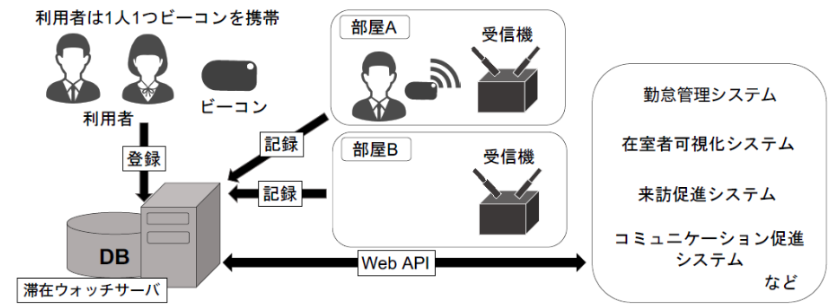
\includegraphics[width=8cm]{image/StayWatch.jpg}
  \caption{「滞在ウォッチ」の概要図}
  \label{multipleBPM}
\end{figure}

%--------------------------------------------
\section{滞在ウォッチ}
\label{sec:const}
本研究のシステム概要を図1に示す.滞在ウォッチは利用者がビーコンを携帯し部屋ごとに設置された受信機によりビーコンを検出する手法で,在室者管理を自動に行う.
サーバには利用者の名前とビーコンのIDを登録する.ビーコンは周囲に数秒に 1回電波を発信する.
受信機が検出したビーコンのIDと電波強度はサーバに送信され,入退室した時刻と日時,在室した部屋名が記録される.


%--------------------------------------------
\section{独立したコミュニティにおける滞在ウォッチの安定運用のためのシステム拡張}
\label{sec:description}

\subsection{受信機データの精度向上}
隣接した部屋の在室判定精度向上と判定誤検知を減らすために受信機データの精度向上を行った.
以前は1度のスキャン終了後にデータを送信する方法を使用していたがビーコンの発進間隔の都合上,全てのビーコンをスキャンするのが難しい場合が存在した.
そこでまず初めに部屋ごとに設置された受信機が一定時間 周辺機器のスキャンを行う.
その後スキャンを数回繰り返しスキャンされたUUIDごとのRSSIの合計値をUUIDごとにスキャンされた回数で割り平均化して送る形を採用した.
ここでの RSSI の合計値とスキャンされた回数は受信機のデータベースに保存しておりサーバ側にデータを送信する際に全てのデータをクリアする.
毎回送信されたデータをサーバ側で複数回受け取りその値を平均化するという手法もあったが処理の複雑化,サーバ側の過剰な負荷の懸念があったためこの方法を採用した.



\subsection{Web ページ閲覧の制限と管理}
在室情報はプライバシーに関わるものであるため複数間コミュニティで適切に扱う必要がある.
そこで Web ページ閲覧者の制限とユーザによる情報公開範囲の変更を行うためにログイン機能の実装を行った.この場合の制限は管理者が登録したユーザのみ閲覧できるものである.ログイン機能には Firebase Authentication,OAuth2.0,Googleアカウント を使用した認証システムを使用している.ユーザ認証システムを独自で実装するという方法もあるが,パスワードのハッシュ化,ハッシュ化に利用している関数の脆弱性,フォームの改竄リスク等,気をつけなければいけないセキュリティリスクがいくつか存在する.Firebase Authentication を利用した実装ならばそれらのリスクを排除できる.

利用ユーザはGoogleアカウントを用いた認証を行うことで新しくIDとPASSWORDを作ることなくページ閲覧が可能である.まずWeb ページ上のログインボタンを押すと Firebase SDK を利用してリダイレクトを行い図5に示すように Google 認証画面に移動する.ここでユーザが許可すると Google の認可サーバがアクセストークンを発行するための認可コードを発行, Web ページにリダイレクトする.リダイレクト時に付与された認可コードを認可サーバに渡すことでアクセストークンを取得する.
次に Web ページから認証 API に対してリクエストを行う.このリクエストはリクエストを送ったユーザが管理者が登録したユーザであるかを確認するために行う.
Webページ側は取得したアクセストークンをHTTP のリクエストヘッダーに付与してリクエストを送る.
認証 API 側はヘッダーからトークンを取得 Firebase Admin SDK を利用してクライアントから送られてきたトークンが正しいユーザのものであるかの検証を行う.
トークン情報が正しくない場合はサーバ側は ステータスコード401,
トークン情報は正しいがトークンから得られるメールアドレスがデータベースに存在しない場合は ステータスコード 403,トークン情報が正しくトークンから得られるメールアドレスが存在する場合は ステータスコード 200 を返す.
Web ページ側は ステータスコード によって適切なコンテンツの表示を切り替えを行っている.



管理者側はユーザの登録を行う.図6に示すように登録フォームでユーザネームと Gmail アドレス,ユーザロールを入力する.
ユーザネームは Web ページで表示される名前である,Gmail アドレスは閲覧を許可する Google アカウントに紐つくメールアドレス,ユーザロールは登録者の権限レベルを表す.
管理者が登録すると該当ユーザのメールアドレスに対して登録が完了したメールが送信される.
メールを受け取ったユーザはログインするとWebページの閲覧が可能となる.



\subsection{BLEビーコンとスマートフォンのハイブリッド化に対応したシステム}
BLEビーコンのアプリケーション化による可用性向上
ユーザの利便性向上のために,BLEビーコンのアプリケーション化をした.
BLEビーコンの導入は容易だが,運用上の諸問題がある.在室判定精度の向上のために,ビーコンは常に動作する必要がある.
しかしBLEビーコンのバッテリー残量の把握は専用のアプリケーションによる接続を要し,バッテリー切れに気が付かなかったユーザや,電池交換を手間に感じたユーザにバッテリー切れを起こしたビーコンが放置される状況が存在した.
これらの問題は,アプリケーション化に伴いハードウェア面,ソフトウェア面から改善がされた.
ハードウェアとして動作するスマートフォンはユーザが高頻度で状態を確認するため,バッテリー切れなど状況の判別が容易である.
また,スマートフォン自体の可用性を維持するために対策を講じるユーザが多く,ビーコンと比較してハードウェアとして可用性が維持されやすい.
ソフトウェア面では,図7に示す通りスマートフォンの通知領域に動作状況を可視化する.通知領域への表示はビーコンとしての動作と連携しており,アプリケーションの動作中は永続的に表示される.
よってアプリケーションが停止した場合もユーザによる判別が容易であるため,アプリケーション再起動によって可用性が維持されやすい.またバックグラウンド動作によってユーザ操作の負担を低減している.
既存のBLEビーコンの利点として正常に動作している限り,ユーザの操作が不要である点が挙げられる.
アプリケーション化に伴い,ユーザの操作が必要になったがそれを最小限に抑えるため,バックグラウンド動作による負担低減を行った.
ユーザの必要な操作は初回のみ必要なログイン処理とビーコン動作の切り替え処理のみである.ログイン処理ではFirebase Authenticationによって登録されたユーザか検証し,データベースからビーコンのデータを取得する.
ビーコン動作の切り替え処理はユーザの事情に応じた選択肢を提供する.在室情報のデータ可用性の観点からは常時のビーコン動作が望ましいが,同時にユーザの使用するスマートフォンのプライバシー性などへの配慮など倫理的課題が存在する.
それらの観点から図8に示すようにビーコン動作の停止が可能になる動作切り替え処理ボタンを提供する.
また,アプリケーション停止時に自動でビーコン動作の復帰が行えないため,ユーザが通知領域で動作していない状態を確認した場合,自らビーコンの動作を開始できる.
\section{今後の課題}
今後の課題として現段階では1つのコミュニティでの運用しかされていないため,実際に複数のコミュニティに導入してもらい,運用を行う必要がある.運用後は,ユーザからの意見や得られたデータを元にシステムの改善を行う予定である.また現状のシステムではコミュニケーションを促進するような仕組みがないためその仕組みづくりを行いたい.

%--------------------------------------------
\begin{thebibliography}{9}
  \bibitem{ura}
  浦正広, 遠藤守, 山田雅之, 宮崎慎也, 岩崎公弥子, 毛利勝廣, 安田孝美, ``天文教育に向けたスマートフォンの活用による対話型の星座検索モデルの提案'', 情報文化学会誌, Vol. 19, No. 2, pp.42--49, 2012.

  \bibitem{tex}
  奥村晴彦, 黒木祐介, ``改訂第6版 \LaTeX2$\epsilon$ 美文書作成入門'', 技術評論社, 2013.

\end{thebibliography}
\end{document}

%%% Local Variables: 
%%% mode: japanese-latex
%%% TeX-master: t
%%% End: 
